\documentclass[12pt]{article}
\usepackage{float}
\usepackage{amsthm}
\usepackage{amsmath}
\usepackage{lineno}
\usepackage{cite}
\usepackage{amssymb,graphics,color,cite,amsmath}
\usepackage{subfig}
\usepackage{graphicx}
\usepackage{epsfig}
\usepackage{psfrag}
\usepackage[margin=0.75in]{geometry}
\usepackage{float}
\usepackage{afterpage}
\usepackage{hyperref}
\usepackage{verbatim}

\usepackage[noblocks]{authblk}
%\usepackage{natbib}
\usepackage{stackengine}

\usepackage{xspace}
\newcommand{\themename}{\textbf{\textsc{metropolis}}\xspace}

\renewcommand{\(}{\left (}
\renewcommand{\)}{\right )}
\renewcommand{\vec}[1]{\boldsymbol{#1}}

\begin{document}

\title{Synchronization of Two Cellular Circadian Rhythms}
\date{}
\author[1]{Yuliang Shi}
\author[2]{Zeshun Zong}
\affil[1,2]{\footnotesize Courant Institute of Mathematical Sciences, New York University, New York}


\maketitle
\begin{abstract}
ABSTRACT
\end{abstract}

\section{Introduction}

\hspace{5mm} Almost all animals have innate biological clock that controls various timing inside the body. Negative feedback of gene expression is one typical generator for a mammalian circadian clock. One simple model of the circadian rhythm is to consider the clock gene expression in a particular cell. This has been shown in Wang and Peskin's work. Building upon their work, we investigate the coupling of two cells with different periods, and study the possible interactions among them.

The model for one cellular circadian oscillator consists of the following: the mRNA and the corresponding proteins encoded by the gene. First, mRNA molecules are synthesized through transcription and enter the cytoplasm. Then, protein molecules are generated in the cytoplasm through translation. Some protein molecules will enter the nucleus and bind to some activating transcription factor on the DNA, thus inhibiting the transcription. This provides a negative feedback that can lean to oscillations in the amount of substances in the cell, provided the parameters are well-chosen.

In this paper we build two such cellular circadian oscillators with different periods. To simulate the information exchange between the two cells, we take a simplified approach that allows protein molecules to directly flow between two cells through diffusion. Both deterministic version and stochastic version of the model are utilized to compare the results.

In the rest of the paper, we first use the deterministic version to find suitable parameters that will generate two oscillations with different periods. Next, we use the deterministic model to study the case when two cells are coupled. Finally, the stochastic version of the model is investigated. Comparisons and analysis are also stated at the end.

\section{Mathematical Modeling}
\subsection{A Simple Cellular Circadian Oscillator}
\hspace{5mm} We construct a four-variable model to simulate the mammalian circadian clock in a cell. This is achieved by the expression of clock gene, e.g. the clock gene \textit{per} in \textit{Drosophila}.

The pathway is shown in Figure 1. The \textit{per} gene is transcribed into \textit{Per} mRNAs in the nucleus, which are then exported to the cytoplasm to be translated to PER protein and to degrade. Some PER proteins enter the nucleus where they inhibit the transcription of the \textit{per} gene and degrade in the nucleus. We assume that the PER proteins inhibit the transcription by binding to the DNA molecules on several pre-determined sites. The transcription continues if and only if none of the sites are occupied.


\begin {figure}[t]
	\centering
	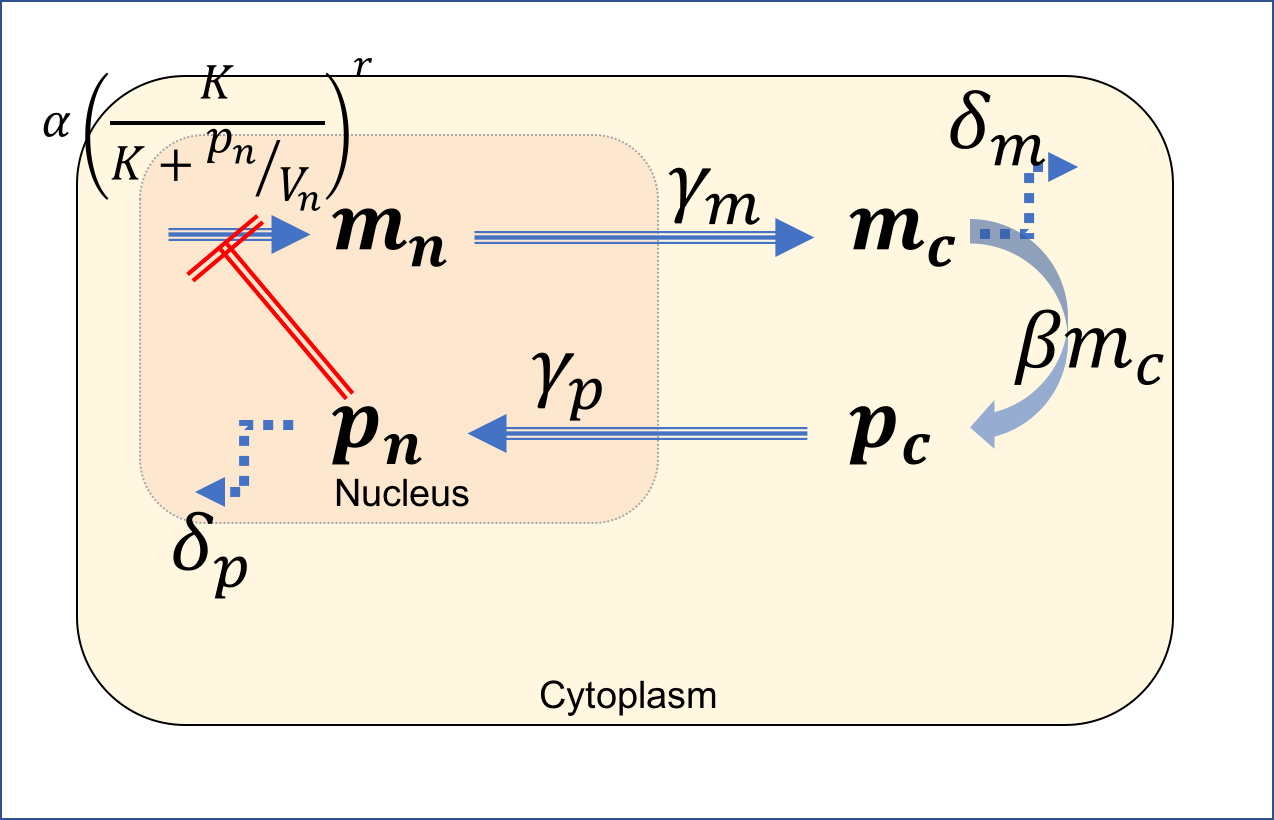
\includegraphics[width=0.5\textwidth]{pathway.png}
	\caption*{\small Figure 1: a schematic cellular clock}
\end {figure}

The variables and parameters that describe the process is the following:
\begin{itemize}
  \item $m_n$: number of mRNAs inside the nucleus;
  \item $m_c$: number of mRNAs in the cytoplasm;
  \item $p_n$: number of protein molecules inside the nucleus;
  \item $p_c$: number of protein molecules in the cytoplasm;
  \item $\alpha$: transcription rate when no proteins are binding;
  \item $r$: total number of sites on which the protein can bind;
  \item $K$: the equilibrium constant of the reaction of protein binding to DNA molecules;
  \item $\gamma_m$: the rate at which mRNAs inside the nucleus are transported to cytoplasm;
  \item $\delta_m$: the degradation rate of mRNAs in cytoplasm;
  \item $\gamma_p$: the rate at which the protein molecules in the cytoplasm are transported into nucleus;
  \item $\delta_p$: the degradation rate of this protein inside nucleus;
	\item $V_n$: the volume of the nucleus.
\end{itemize}

Using the above notations, we can define the six reactions involved in the model in Table 1. One remark is that the rate of transcription is $\alpha \{\frac{K}{K + p_n / V_n}\}^r.$ We can think of $\frac{K}{K + p_n / V_n}$ as the possibility that one particular site is not occupied, so it being raised to $r^\text{th}$ power is the probability that all sites are not occupied. The deduction of this expression can be found in Wang and Peskin's work.

\begin{table}[t]
\begin{tabular}{|l|l|l|l|}
\hline
Reaction  & Reaction Name                            & Rate (Probability)                     & Result                                                                         \\ \hline
1          & Transcription of the gene                & $\alpha \{\frac{K}{K + p_n / V_n}\}^r$ & $m_n \to m_n +1$                                                               \\ \hline
2          & Export of mRNA from nucleus to cytoplasm & $\gamma_m m_n$                         & \begin{tabular}[c]{@{}l@{}}$m_n \to m_n -1,$\\ $m_c \to m_c +1$\end{tabular}   \\ \hline
3          & Translation of the mRNA                  & $\beta m_c$                            & $p_c \to p_c + 1$                                                              \\ \hline
4          & Import of protein into nucleus           & $\gamma_p p_c$                         & \begin{tabular}[c]{@{}l@{}}$p_c \to p_c - 1,$\\ $p_n \to p_n + 1$\end{tabular} \\ \hline
5          & Degradation of mRNA in cytoplasm         & $\delta_m m_c$                         & $m_c \to m_c -1$                                                               \\ \hline
6          & Degradation of protein in nucleus        & $\delta_p p_n$                         & $p_n \to p_n -1$                                                               \\ \hline
\end{tabular}
\caption*{\small Table 1: Reaction Table}
\end{table}
The model consists of two versions.
\subsection{Deterministic Version}
\hspace{5mm} If we view the number of molecules of each substance as large numbers, the fact that them being integers will have little influence on the model. In this way, we can set up the model using differential equations. Notice that the rate of change of the amount of one substance is equal to the rate that it is produced (imported) minus the rate that it is degraded (exported). This gives us the following:
\begin{equation}
	\frac{dm_n}{dt} = \alpha \{\frac{K}{K + p_n / V_n}\}^r - \delta_m m_n,
\end{equation}

\begin{equation}
	\frac{dm_c}{dt} = \gamma_m m_n - \delta_m m_c,
\end{equation}

\begin{equation}
	\frac{dp_c}{dt} = \beta m_c - \gamma_p p_c,
\end{equation}

\begin{equation}
	\frac{dp_n}{dt} = \gamma_p p_c - \delta_p p_n.
\end{equation}

If we write $k = K V_n,$ then the first equation becomes $\frac{dm_n}{dt} = \alpha \{\frac{k}{k + p_n}\}^r - \delta_m m_n.$ Hence the set of differential equations can also be written as
\begin{equation}
	\frac{dm_n}{dt} = \alpha \{\frac{k}{k + p_n}\}^r - \delta_m m_n,
\end{equation}

\begin{equation}
	\frac{dm_c}{dt} = \gamma_m m_n - \delta_m m_c,
\end{equation}

\begin{equation}
	\frac{dp_c}{dt} = \beta m_c - \gamma_p p_c,
\end{equation}

\begin{equation}
	\frac{dp_n}{dt} = \gamma_p p_c - \delta_p p_n.
\end{equation}

Here we state that, besides modeling, the set of equations can also give insight on the choice of parameters in order to yield an expected oscillation. This is discussed later.


\subsection{Stochastic (Microscopic) Version}
\hspace{5mm} On the other hand, we can also look at the microscopic version, keeping track of the number of each molecules when each reaction happens. Recall that if an event has probability per unit time $r$ to happen, and let $T$ denote the time this event first happens, then
\begin{equation}
	\mathbb{P}(T > t) = \lim_{n \to \infty} \prod_{j=1}^{n} (1-\frac{rt}{n}) = \lim_{n \to \infty} (1 - \frac{rt}{n})^n = e^{-rt}.
\end{equation}
So $T$ follows an exponential distribution with parameter $r.$  Since $T$ is continuous, it follows that $F(T),$ the distribution function acting on $T,$ is uniformly distributed on the interval $(0,1).$ Hence, $$-\frac{\log(U)}{r},$$ with $U$ being a random variable uniformly distributed on the interval $(0,1),$ would generate a realization of $T.$

In the stochastic approach, given initial amount of each substances, six reaction times (each follows an exponential distribution with the parameter being the reaction's probability per unit time, respectively) are generated. We assume only the first reaction actually happens. Then the numbers of molecules are adjusted correspondingly and the above process is repeated.

\begin{thebibliography}{9}

	\bibitem{gyrocom}
	Charles S. Peskin. (2018).
	Notes on gyrocompass.

	\bibitem{rbm}
	Charles Puelz. (2018).
	Matlab code about rigid body motion.




\end{thebibliography}

\end{document}
